\section{Conclusions}

The project provides results which are a promising sign towards implementing image alignment techniques using lightweight fuzzy entropy algorithms. The results show a varied output of aligned \gls{mammographic images}, each usually maintaining a natural shape.

\subsection{Does the use of fuzzy entropy alignment metrics improve the alignment of mammograms?}

The judgement as to whether the fuzzy entropy metrics align images `better' than standard Shannon entropy is a subjective one. However this project does show that the output gained from fuzzy entropy \gls{Congealing} is somewhat different to that of Shannon entropy due to the uncertainty introduced via fuzzy set theory, and therefore could be perceived to be more useful to a mammographer.

Figure \ref{fig:comparison-of-techniques} presents the three different entropy-based alignment metrics, running the same amount of iterations and upon the same dataset.

\begin{figure}[H]
    \centering
    \begin{subfigure}[t]{0.3\textwidth}
        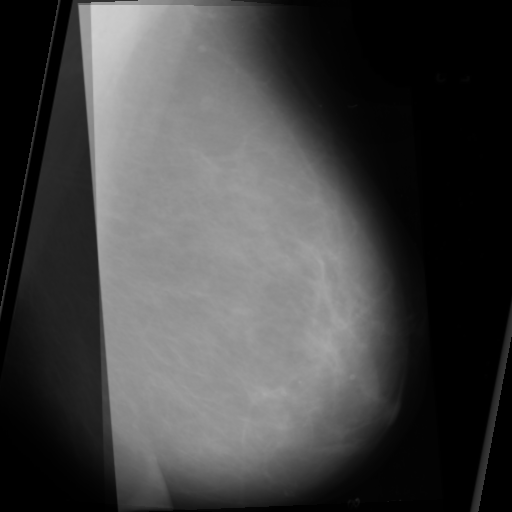
\includegraphics[width=\textwidth]{Chapter3/shannon-img/s-10-final.png}
        \caption{10 Shannon entropy iterations.}
        \label{fig:shannon-comp}
    \end{subfigure} \hfill
    ~ %add desired spacing between images, e. g. ~, \quad, \qquad, \hfill etc.
      %(or a blank line to force the subfigure onto a new line)
    \begin{subfigure}[t]{0.3\textwidth}
        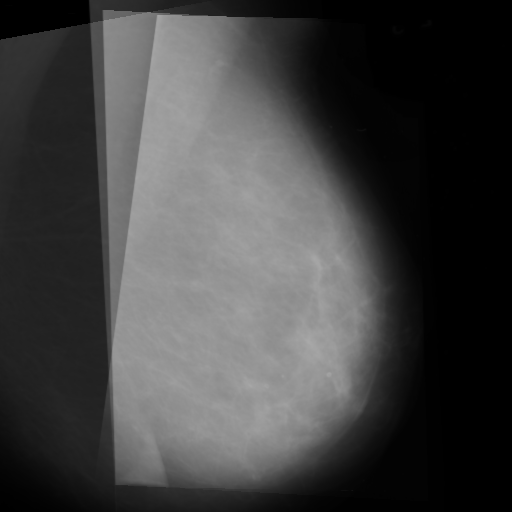
\includegraphics[width=\textwidth]{Chapter3/nonProb-img/nonprob10.png}
        \caption{10 Non-Probabilistic entropy iterations.}
        \label{fig:nonProb-comp}
    \end{subfigure} \hfill
    \begin{subfigure}[t]{0.3\textwidth}
      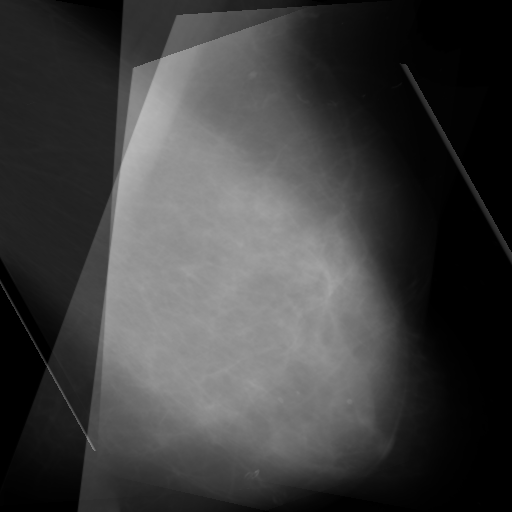
\includegraphics[width=\textwidth]{Chapter3/hybrid-img/hybrid-10.png}
      \caption{10 Hybrid entropy iterations.}
      \label{fig:hybrid-comp}
    \end{subfigure}
    \caption{Comparison of the three entropy alignment metrics upon Set 1 - BI-RADS I image data.}
    \label{fig:comparison-of-techniques}
\end{figure}

\subsection{Do mammographers find the output at all useful?}

Unfortunately due to the time constraints of this project, the author was unable to ascertain a firm conclusion to this hypothesis. It is hoped that given the appropriate nature of the outputs produced, that this work would indeed be useful to mammographers in their classification of breast tissue density, as it provides a generalised average image of each BI-RADS density classification.

\subsection{What advantages / disadvantages does each entropy alignment metric entail?}

\subsubsection{Shannon entropy}

\textbf{Advantages: }
The Shannon entropy implementation provided by Learned-Miller has the quickest performance rate due to the lookup table implementation, and straightforward mathematics involved. Combining this with the sensible output the user can expect after 20+ iterations, makes this an extremely strong benchmark for the two fuzzy entropy implementations.

\textbf{Disadvantages: }
However, this project was about utilising uncertainty and using it to model breast tissue accurately. Shannon entropy provides no such uncertainty, and therefore the alignment of the images is based purely on the condition that pixels match one another exactly, with no variation allowed. This rigidity can translate into a slower alignment process.

\subsubsection{Non-Probabilistic entropy}

\textbf{Advantages}
At 20 iterations, Non-Probabilistic entropy can be seen in some experiments to be \say{over-congealing} the input images, yet the output images were never corrupted nor distorted. This natural slowing on entropy decline, with fluctuating results in the latter stages is extremely reflective of nature. Were a human try to align two images by hand, their initial results would see large changes in alignment, however the more precise they try to be, the more the alignment is likely to just miss the mark.

This alignment metric exhibits a quick decrease in entropy in the first few iterations of the \Gls{Congealing} algorithm. This results in fewer iterations necessary for an accurate alignment when compared to it`s counterparts.

\noindent \textbf{Disadvantages}
Whilst the metric takes very few iterations to align the input images accurately, the performance of this implementation is not ideal. With run-times up to 4830\% longer (\textit{1.22 vs 58.93 seconds per iteration}) than that of Shannon entropy, as seen in Table \ref{table:run-time}, it is by no means a quick solution. This could be due to implementation, however the final run-times produced for Non-Probabilistic entropy are inclusive of the vectorisation optimisations carried out during implementation. Prior to vectorisation run-times were significantly worse, as detailed in Subsection \ref{ssec:vectorisation}.

As the algorithm name suggests, this fuzzy entropy metric does not model probabilistic uncertainty, just that of possibilistic, therefore does not model true uncertainty to the same level as Hybrid entropy.

\subsubsection{Hybrid entropy}

\noindent \textbf{Advantages}
The run-times produced by Hybrid entropy are close to that of Shannon entropy's. This is admirable given the complexity of the calculations involved in the generation of the input image entropy value. This quick run-time brings to the user a truly usable image alignment method which leverages fuzzy entropy.

Whilst the entropy was often not as small as that output by Non-Probabilistic entropy, it produced an admirable attempt at initially aligning the input images, and went on to produce the highest degradations in entropy seen in this project.

\noindent \textbf{Disadvantages}

One issue faced by Hybrid entropy was over-congealing. Whilst the entropy value did not indicate a value near over-congealment, the image output afterwards did cause some concern. As mentioned previously (Subsection \ref{sssec:hybrid-alignment}), estimating when to cut off Hybrid entropy is difficult, as over-congealment often happened at varying iterations given different data-sets.

\subsection{Future Advancements}
\label{ssec:improvements}

Several features were identified for improvement, plus additional functionality could be added to the project if the project time frame had been longer, or if this project were to be continued at a later stage.

\subsubsection{Automated medical marker removal}
Feature extraction is an ongoing research area. This could be leveraged in the future for the automatic detection and removal of medical markers and/or artefacts. Some interesting areas of research which may be viable for implementation include:

\noindent \textbf{Corner detection: } As the artefacts are typically rectangular in shape, a corner detector could be used to identify their presence - such as Harris Corners, or KLT. Harris Corners was developed by Chris Harris and Mike Stephens in 1988, in a technique which combines an edge detector with a corner detector \cite{Harris_Stephens_1988}. Harris Corners algorithm is looking for a sharp change in intensity within the image, such as passing from the black mammogram background onto the white area of the artefact. If a right-angle in intensity difference can be detected using several sliding windows over the image, then a corner is detected.

The work of Kanade-Lucas-Tomasi on the self-titled algorithm \acrshort{KLT} builds upon that of Harris and Stephens \cite{Shi_Tomasi_1994} \cite{tomasi2004detection}. This implements a scoring function where the highest value (e.g. $x$) above a threshold are classed as a corner, and all other values which neighbour $x$ are removed from contention.

When compared, both Harris and KLT corners perform very similarly and are both still regularly used today.

\noindent \textbf{SURF: } \acrfull{SURF} \cite{Bay_Tuytelaars_Gool_2006} is a speeded up version of an older feature extraction method called \acrfull{SIFT} \cite{Lowe_1999}. \acrshort{SIFT} boasts a number of useful features such as being scale invariant (useful as not all artefacts are the same size), invariant to rotation (again useful as artefacts are often at different orientations) and features are selected only if there is a good enough contrast (as artefacts are typically white on a black background, this is helpful). \acrshort{SURF} improves upon \acrshort{SIFT} by utilising different-sized box features rather than \acrfull{DOG} filters for refining the space in which scale is analysed, therefore making it quicker.

\subsubsection{Classify unseen mammographic images}

If further work was undertaken to build upon this project, the application could be used to classify new, unseen \gls{mammographic images} into the correct BI-RADS classification using some kind of Machine Learning method. The application could be trained upon the existing Mini-MIAS dataset \cite{Suckling_1994}, along with other datasets which contain healthy tissue, such as \acrshort{DDSM} \cite{Heath_Bowyer_Kopans_Moore_Kegelmeyer_Processing} \cite{Heath_Bowyer_Kopans_Kegelmeyer_Moore_Chang_MunishKumaran_1998} to create an accurate model of what each classification should tend towards.

Research is ongoing into which Machine Learning technique is the best for classification of images, however the likely choice would be either an Artificial Neural Network (ANN) or a Support Vector Machine (SVN) given their high accuracy rate, as outlined in \cite{kotsiantis2007supervised}. Currently both of these are slow to train, however that wouldn't necessarily be a problem for a Doctor to deal with, as it could be trained prior to their usage, or trained annually on new available data to become even more accurate. A high accuracy rate is more important than the training rate due to the human-diagnosis element of the application.

\subsubsection{Optimisation of Non-Probabilistic}

The functionality to run all 3 alignment metrics together was not implemented due to the performance issue of Non-Probabilistic entropy, however if further work was done to optimise the performance, then the author can see no issue as to why all three alignment metrics could be run, and the results displayed side-by-side for comparison.

The current implementation means the user would have to run the three alignment techniques sequentially, the outputs saved to their PC, and then later opened in an image preview software to compare the results alongside each other. This is not a major issue, however it would be advantageous if the user could view them side-by-side easily.

\subsubsection{Further optimisation}

Further optimisation could be carried out for the two fuzzy entropy algorithms by implementing a lookup table structure, as in Learned-Miller's example of Shannon entropy. Whilst this is unlikely to make massive gains for Hybrid entropy, for Non-Probabilistic entropy this could see a significant reduction in run-time, making the algorithm more usable in real-world environments.

\subsubsection{GUI alterations}

Small edits would be made to the \texttt{removeMarker} \acrshort{GUI}, such as a clear button, and the functionality to draw more than one area to remove from an image.

The load functionality in the main \acrshort{GUI} could be compiled into one button - this was initially attempted during the project, however a lack of knowledge into how to detect if a file already exists, along with time constraints, inhibited this advancement.
